\documentclass[12pt]{article} 
% \documentclass[12pt]{amsart} 

% Custom definitions
% To use this customization file, insert the line "% Custom definitions
% To use this customization file, insert the line "% Custom definitions
% To use this customization file, insert the line "\input{custom}" in the header of the tex file.

% Formatting

\tolerance=1000
\usepackage[margin=1in]{geometry}


% Packages

% \usepackage{amssymb,latexsym}
\usepackage{amssymb,amsfonts,amsmath,latexsym,amsthm}
\usepackage[usenames,dvipsnames]{color}
\usepackage[]{graphicx}
\usepackage[space]{grffile}
\usepackage{mathrsfs}   % fancy math font
% \usepackage[font=small,skip=0pt]{caption}
\usepackage[skip=0pt]{caption}
\usepackage{subcaption}
\usepackage{verbatim}
\usepackage{url}
\usepackage{bm}
\usepackage{dsfont}
\usepackage{extarrows}
\usepackage{multirow}
% \usepackage{wrapfig}
% \usepackage{epstopdf}
\usepackage{rotating}
\usepackage{tikz}
\usetikzlibrary{fit}					% fitting shapes to coordinates
%\usetikzlibrary{backgrounds}	% drawing the background after the foreground

\usepackage{fancyhdr}

\fancypagestyle{firststyle}{
   \fancyhf{}
   \renewcommand{\footrulewidth}{0.4pt}
   \fancyfoot[L]{\footnotesize This work is licensed under a \href{http://creativecommons.org/licenses/by-nc-nd/4.0/}{Creative Commons BY-NC-ND 4.0 International License}.\\ Jeffrey W. Miller (2015). \textit{Lecture Notes on Bayesian Statistics}. Duke University, Durham, NC.}
}


% \usepackage[dvipdfm,colorlinks,citecolor=blue,linkcolor=blue,urlcolor=blue]{hyperref}
\usepackage[colorlinks,citecolor=blue,linkcolor=blue,urlcolor=blue]{hyperref}
%\usepackage{hyperref}
\usepackage[authoryear,round]{natbib}


%  Theorems, etc.

\theoremstyle{plain}
\newtheorem{theorem}{Theorem}[section]
\newtheorem{corollary}[theorem]{Corollary}
\newtheorem{lemma}[theorem]{Lemma}
\newtheorem{proposition}[theorem]{Proposition}
\newtheorem{condition}[theorem]{Condition}
% \newtheorem{conditions}[theorem]{Conditions}

\theoremstyle{definition}
\newtheorem{definition}[theorem]{Definition}
% \newtheorem*{unnumbered-definition}{Definition}
\newtheorem{example}[theorem]{Example}
\theoremstyle{remark}
\newtheorem*{remark}{Remark}
\numberwithin{equation}{section}



% Document-specific shortcuts
\newcommand{\btheta}{{\bm\theta}}
\newcommand{\bbtheta}{{\pmb{\bm\theta}}}

\newcommand{\commentary}[1]{\ifx\showcommentary\undefined\else \emph{#1}\fi}

\newcommand{\term}[1]{\textit{\textbf{#1}}}

% Math shortcuts

% Probability distributions
\DeclareMathOperator*{\Exp}{Exp}
\DeclareMathOperator*{\TExp}{TExp}
\DeclareMathOperator*{\Bernoulli}{Bernoulli}
\DeclareMathOperator*{\Beta}{Beta}
\DeclareMathOperator*{\Ga}{Gamma}
\DeclareMathOperator*{\TGamma}{TGamma}
\DeclareMathOperator*{\Poisson}{Poisson}
\DeclareMathOperator*{\Binomial}{Binomial}
\DeclareMathOperator*{\NormalGamma}{NormalGamma}
\DeclareMathOperator*{\InvGamma}{InvGamma}
\DeclareMathOperator*{\Cauchy}{Cauchy}
\DeclareMathOperator*{\Uniform}{Uniform}
\DeclareMathOperator*{\Gumbel}{Gumbel}
\DeclareMathOperator*{\Pareto}{Pareto}
\DeclareMathOperator*{\Mono}{Mono}
\DeclareMathOperator*{\Geometric}{Geometric}
\DeclareMathOperator*{\Wishart}{Wishart}

% Math operators
\DeclareMathOperator*{\argmin}{arg\,min}
\DeclareMathOperator*{\argmax}{arg\,max}
\DeclareMathOperator*{\Cov}{Cov}
\DeclareMathOperator*{\diag}{diag}
\DeclareMathOperator*{\median}{median}
\DeclareMathOperator*{\Vol}{Vol}

% Math characters
\newcommand{\R}{\mathbb{R}}
\newcommand{\Z}{\mathbb{Z}}
\newcommand{\E}{\mathbb{E}}
\renewcommand{\Pr}{\mathbb{P}}
\newcommand{\I}{\mathds{1}}
\newcommand{\V}{\mathbb{V}}

\newcommand{\A}{\mathcal{A}}
\newcommand{\C}{\mathcal{C}}
\newcommand{\D}{\mathcal{D}}
\newcommand{\Hcal}{\mathcal{H}}
\newcommand{\M}{\mathcal{M}}
\newcommand{\N}{\mathcal{N}}
\newcommand{\X}{\mathcal{X}}
\newcommand{\Zcal}{\mathcal{Z}}
\renewcommand{\P}{\mathcal{P}}

\newcommand{\T}{\mathtt{T}}
\renewcommand{\emptyset}{\varnothing}


% Miscellaneous commands
\newcommand{\iid}{\stackrel{\mathrm{iid}}{\sim}}
\newcommand{\matrixsmall}[1]{\bigl(\begin{smallmatrix}#1\end{smallmatrix} \bigr)}

\newcommand{\items}[1]{\begin{itemize} #1 \end{itemize}}

\newcommand{\todo}[1]{\emph{\textcolor{red}{(#1)}}}

\newcommand{\branch}[4]{
\left\{
	\begin{array}{ll}
		#1  & \mbox{if } #2 \\
		#3 & \mbox{if } #4
	\end{array}
\right.
}

% approximately proportional to
\def\app#1#2{%
  \mathrel{%
    \setbox0=\hbox{$#1\sim$}%
    \setbox2=\hbox{%
      \rlap{\hbox{$#1\propto$}}%
      \lower1.3\ht0\box0%
    }%
    \raise0.25\ht2\box2%
  }%
}
\def\approxprop{\mathpalette\app\relax}

% \newcommand{\approptoinn}[2]{\mathrel{\vcenter{
  % \offinterlineskip\halign{\hfil$##$\cr
    % #1\propto\cr\noalign{\kern2pt}#1\sim\cr\noalign{\kern-2pt}}}}}

% \newcommand{\approxpropto}{\mathpalette\approptoinn\relax}





" in the header of the tex file.

% Formatting

\tolerance=1000
\usepackage[margin=1in]{geometry}


% Packages

% \usepackage{amssymb,latexsym}
\usepackage{amssymb,amsfonts,amsmath,latexsym,amsthm}
\usepackage[usenames,dvipsnames]{color}
\usepackage[]{graphicx}
\usepackage[space]{grffile}
\usepackage{mathrsfs}   % fancy math font
% \usepackage[font=small,skip=0pt]{caption}
\usepackage[skip=0pt]{caption}
\usepackage{subcaption}
\usepackage{verbatim}
\usepackage{url}
\usepackage{bm}
\usepackage{dsfont}
\usepackage{extarrows}
\usepackage{multirow}
% \usepackage{wrapfig}
% \usepackage{epstopdf}
\usepackage{rotating}
\usepackage{tikz}
\usetikzlibrary{fit}					% fitting shapes to coordinates
%\usetikzlibrary{backgrounds}	% drawing the background after the foreground

\usepackage{fancyhdr}

\fancypagestyle{firststyle}{
   \fancyhf{}
   \renewcommand{\footrulewidth}{0.4pt}
   \fancyfoot[L]{\footnotesize This work is licensed under a \href{http://creativecommons.org/licenses/by-nc-nd/4.0/}{Creative Commons BY-NC-ND 4.0 International License}.\\ Jeffrey W. Miller (2015). \textit{Lecture Notes on Bayesian Statistics}. Duke University, Durham, NC.}
}


% \usepackage[dvipdfm,colorlinks,citecolor=blue,linkcolor=blue,urlcolor=blue]{hyperref}
\usepackage[colorlinks,citecolor=blue,linkcolor=blue,urlcolor=blue]{hyperref}
%\usepackage{hyperref}
\usepackage[authoryear,round]{natbib}


%  Theorems, etc.

\theoremstyle{plain}
\newtheorem{theorem}{Theorem}[section]
\newtheorem{corollary}[theorem]{Corollary}
\newtheorem{lemma}[theorem]{Lemma}
\newtheorem{proposition}[theorem]{Proposition}
\newtheorem{condition}[theorem]{Condition}
% \newtheorem{conditions}[theorem]{Conditions}

\theoremstyle{definition}
\newtheorem{definition}[theorem]{Definition}
% \newtheorem*{unnumbered-definition}{Definition}
\newtheorem{example}[theorem]{Example}
\theoremstyle{remark}
\newtheorem*{remark}{Remark}
\numberwithin{equation}{section}



% Document-specific shortcuts
\newcommand{\btheta}{{\bm\theta}}
\newcommand{\bbtheta}{{\pmb{\bm\theta}}}

\newcommand{\commentary}[1]{\ifx\showcommentary\undefined\else \emph{#1}\fi}

\newcommand{\term}[1]{\textit{\textbf{#1}}}

% Math shortcuts

% Probability distributions
\DeclareMathOperator*{\Exp}{Exp}
\DeclareMathOperator*{\TExp}{TExp}
\DeclareMathOperator*{\Bernoulli}{Bernoulli}
\DeclareMathOperator*{\Beta}{Beta}
\DeclareMathOperator*{\Ga}{Gamma}
\DeclareMathOperator*{\TGamma}{TGamma}
\DeclareMathOperator*{\Poisson}{Poisson}
\DeclareMathOperator*{\Binomial}{Binomial}
\DeclareMathOperator*{\NormalGamma}{NormalGamma}
\DeclareMathOperator*{\InvGamma}{InvGamma}
\DeclareMathOperator*{\Cauchy}{Cauchy}
\DeclareMathOperator*{\Uniform}{Uniform}
\DeclareMathOperator*{\Gumbel}{Gumbel}
\DeclareMathOperator*{\Pareto}{Pareto}
\DeclareMathOperator*{\Mono}{Mono}
\DeclareMathOperator*{\Geometric}{Geometric}
\DeclareMathOperator*{\Wishart}{Wishart}

% Math operators
\DeclareMathOperator*{\argmin}{arg\,min}
\DeclareMathOperator*{\argmax}{arg\,max}
\DeclareMathOperator*{\Cov}{Cov}
\DeclareMathOperator*{\diag}{diag}
\DeclareMathOperator*{\median}{median}
\DeclareMathOperator*{\Vol}{Vol}

% Math characters
\newcommand{\R}{\mathbb{R}}
\newcommand{\Z}{\mathbb{Z}}
\newcommand{\E}{\mathbb{E}}
\renewcommand{\Pr}{\mathbb{P}}
\newcommand{\I}{\mathds{1}}
\newcommand{\V}{\mathbb{V}}

\newcommand{\A}{\mathcal{A}}
\newcommand{\C}{\mathcal{C}}
\newcommand{\D}{\mathcal{D}}
\newcommand{\Hcal}{\mathcal{H}}
\newcommand{\M}{\mathcal{M}}
\newcommand{\N}{\mathcal{N}}
\newcommand{\X}{\mathcal{X}}
\newcommand{\Zcal}{\mathcal{Z}}
\renewcommand{\P}{\mathcal{P}}

\newcommand{\T}{\mathtt{T}}
\renewcommand{\emptyset}{\varnothing}


% Miscellaneous commands
\newcommand{\iid}{\stackrel{\mathrm{iid}}{\sim}}
\newcommand{\matrixsmall}[1]{\bigl(\begin{smallmatrix}#1\end{smallmatrix} \bigr)}

\newcommand{\items}[1]{\begin{itemize} #1 \end{itemize}}

\newcommand{\todo}[1]{\emph{\textcolor{red}{(#1)}}}

\newcommand{\branch}[4]{
\left\{
	\begin{array}{ll}
		#1  & \mbox{if } #2 \\
		#3 & \mbox{if } #4
	\end{array}
\right.
}

% approximately proportional to
\def\app#1#2{%
  \mathrel{%
    \setbox0=\hbox{$#1\sim$}%
    \setbox2=\hbox{%
      \rlap{\hbox{$#1\propto$}}%
      \lower1.3\ht0\box0%
    }%
    \raise0.25\ht2\box2%
  }%
}
\def\approxprop{\mathpalette\app\relax}

% \newcommand{\approptoinn}[2]{\mathrel{\vcenter{
  % \offinterlineskip\halign{\hfil$##$\cr
    % #1\propto\cr\noalign{\kern2pt}#1\sim\cr\noalign{\kern-2pt}}}}}

% \newcommand{\approxpropto}{\mathpalette\approptoinn\relax}





" in the header of the tex file.

% Formatting

\tolerance=1000
\usepackage[margin=1in]{geometry}


% Packages

% \usepackage{amssymb,latexsym}
\usepackage{amssymb,amsfonts,amsmath,latexsym,amsthm}
\usepackage[usenames,dvipsnames]{color}
\usepackage[]{graphicx}
\usepackage[space]{grffile}
\usepackage{mathrsfs}   % fancy math font
% \usepackage[font=small,skip=0pt]{caption}
\usepackage[skip=0pt]{caption}
\usepackage{subcaption}
\usepackage{verbatim}
\usepackage{url}
\usepackage{bm}
\usepackage{dsfont}
\usepackage{extarrows}
\usepackage{multirow}
% \usepackage{wrapfig}
% \usepackage{epstopdf}
\usepackage{rotating}
\usepackage{tikz}
\usetikzlibrary{fit}					% fitting shapes to coordinates
%\usetikzlibrary{backgrounds}	% drawing the background after the foreground

\usepackage{fancyhdr}

\fancypagestyle{firststyle}{
   \fancyhf{}
   \renewcommand{\footrulewidth}{0.4pt}
   \fancyfoot[L]{\footnotesize This work is licensed under a \href{http://creativecommons.org/licenses/by-nc-nd/4.0/}{Creative Commons BY-NC-ND 4.0 International License}.\\ Jeffrey W. Miller (2015). \textit{Lecture Notes on Bayesian Statistics}. Duke University, Durham, NC.}
}


% \usepackage[dvipdfm,colorlinks,citecolor=blue,linkcolor=blue,urlcolor=blue]{hyperref}
\usepackage[colorlinks,citecolor=blue,linkcolor=blue,urlcolor=blue]{hyperref}
%\usepackage{hyperref}
\usepackage[authoryear,round]{natbib}


%  Theorems, etc.

\theoremstyle{plain}
\newtheorem{theorem}{Theorem}[section]
\newtheorem{corollary}[theorem]{Corollary}
\newtheorem{lemma}[theorem]{Lemma}
\newtheorem{proposition}[theorem]{Proposition}
\newtheorem{condition}[theorem]{Condition}
% \newtheorem{conditions}[theorem]{Conditions}

\theoremstyle{definition}
\newtheorem{definition}[theorem]{Definition}
% \newtheorem*{unnumbered-definition}{Definition}
\newtheorem{example}[theorem]{Example}
\theoremstyle{remark}
\newtheorem*{remark}{Remark}
\numberwithin{equation}{section}



% Document-specific shortcuts
\newcommand{\btheta}{{\bm\theta}}
\newcommand{\bbtheta}{{\pmb{\bm\theta}}}

\newcommand{\commentary}[1]{\ifx\showcommentary\undefined\else \emph{#1}\fi}

\newcommand{\term}[1]{\textit{\textbf{#1}}}

% Math shortcuts

% Probability distributions
\DeclareMathOperator*{\Exp}{Exp}
\DeclareMathOperator*{\TExp}{TExp}
\DeclareMathOperator*{\Bernoulli}{Bernoulli}
\DeclareMathOperator*{\Beta}{Beta}
\DeclareMathOperator*{\Ga}{Gamma}
\DeclareMathOperator*{\TGamma}{TGamma}
\DeclareMathOperator*{\Poisson}{Poisson}
\DeclareMathOperator*{\Binomial}{Binomial}
\DeclareMathOperator*{\NormalGamma}{NormalGamma}
\DeclareMathOperator*{\InvGamma}{InvGamma}
\DeclareMathOperator*{\Cauchy}{Cauchy}
\DeclareMathOperator*{\Uniform}{Uniform}
\DeclareMathOperator*{\Gumbel}{Gumbel}
\DeclareMathOperator*{\Pareto}{Pareto}
\DeclareMathOperator*{\Mono}{Mono}
\DeclareMathOperator*{\Geometric}{Geometric}
\DeclareMathOperator*{\Wishart}{Wishart}

% Math operators
\DeclareMathOperator*{\argmin}{arg\,min}
\DeclareMathOperator*{\argmax}{arg\,max}
\DeclareMathOperator*{\Cov}{Cov}
\DeclareMathOperator*{\diag}{diag}
\DeclareMathOperator*{\median}{median}
\DeclareMathOperator*{\Vol}{Vol}

% Math characters
\newcommand{\R}{\mathbb{R}}
\newcommand{\Z}{\mathbb{Z}}
\newcommand{\E}{\mathbb{E}}
\renewcommand{\Pr}{\mathbb{P}}
\newcommand{\I}{\mathds{1}}
\newcommand{\V}{\mathbb{V}}

\newcommand{\A}{\mathcal{A}}
\newcommand{\C}{\mathcal{C}}
\newcommand{\D}{\mathcal{D}}
\newcommand{\Hcal}{\mathcal{H}}
\newcommand{\M}{\mathcal{M}}
\newcommand{\N}{\mathcal{N}}
\newcommand{\X}{\mathcal{X}}
\newcommand{\Zcal}{\mathcal{Z}}
\renewcommand{\P}{\mathcal{P}}

\newcommand{\T}{\mathtt{T}}
\renewcommand{\emptyset}{\varnothing}


% Miscellaneous commands
\newcommand{\iid}{\stackrel{\mathrm{iid}}{\sim}}
\newcommand{\matrixsmall}[1]{\bigl(\begin{smallmatrix}#1\end{smallmatrix} \bigr)}

\newcommand{\items}[1]{\begin{itemize} #1 \end{itemize}}

\newcommand{\todo}[1]{\emph{\textcolor{red}{(#1)}}}

\newcommand{\branch}[4]{
\left\{
	\begin{array}{ll}
		#1  & \mbox{if } #2 \\
		#3 & \mbox{if } #4
	\end{array}
\right.
}

% approximately proportional to
\def\app#1#2{%
  \mathrel{%
    \setbox0=\hbox{$#1\sim$}%
    \setbox2=\hbox{%
      \rlap{\hbox{$#1\propto$}}%
      \lower1.3\ht0\box0%
    }%
    \raise0.25\ht2\box2%
  }%
}
\def\approxprop{\mathpalette\app\relax}

% \newcommand{\approptoinn}[2]{\mathrel{\vcenter{
  % \offinterlineskip\halign{\hfil$##$\cr
    % #1\propto\cr\noalign{\kern2pt}#1\sim\cr\noalign{\kern-2pt}}}}}

% \newcommand{\approxpropto}{\mathpalette\approptoinn\relax}






\setcounter{tocdepth}{1}
%\usepackage{caption}

\graphicspath{{figures/}}

% Start doing this:
%
% "You need to follow the guidelines set by the license. I'm only going to address attribution. According to Creative Commons you need to:
% 1. keep intact any copyright notices for the Work
% 2. credit the author, licensor and/or other parties (such as a wiki or journal) in the manner they specify;
% 3. include the title of the Work
% 4. the URL for the work if applicable
% 5. If you are making a derivative word or adaptation, in addition to the above, you need to identify that your work is a derivative work i.e., 'This is a Finnish translation of the [original work] by [author].' or 'Screenplay based on [original work] by [author].'
%
% http://librarianbyday.net/2009/09/28/how-to-attribute-a-creative-commons-photo-from-flickr/
% https://wiki.creativecommons.org/Best_practices_for_attribution


\title{Chapter 2: Background and Motivation}
\author{}
\date{}

\def\showcommentary{1}

\begin{document}
\maketitle
{\footnotesize
\tableofcontents 
}
\thispagestyle{firststyle}

\vspace{3em}

\section{Applications of Bayesian statistics}

There are many real-world applications where Bayesian statistics is used in practice. Below are some prominent and/or interesting examples. Of course, one could just as easily come up with a list of applications where non-Bayesian methods are used, but the focus here is on Bayesian statistics.

\subsection{Tracking}


\begin{figure}
    \centering
    \begin{subfigure}[t]{0.48\textwidth}
        \centering
        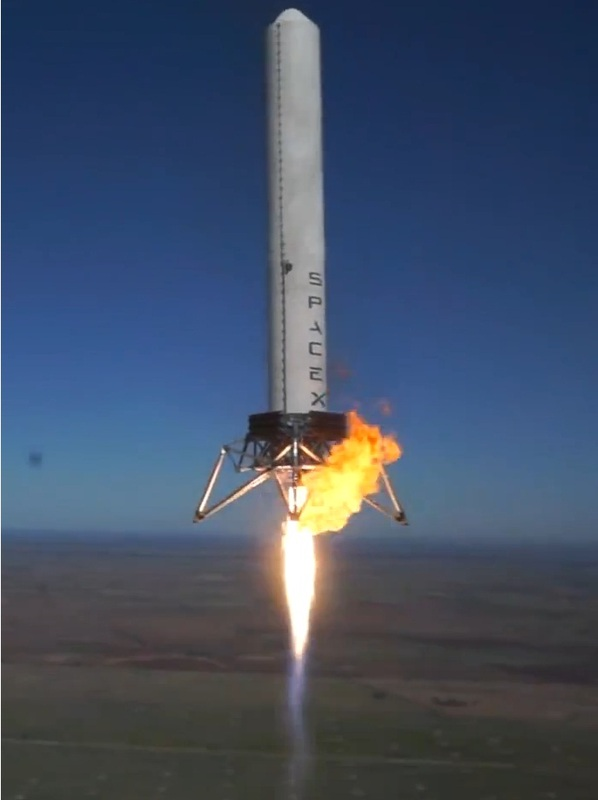
\includegraphics[height=2in]{spacex.jpg}
        % http://www.spaceflight101.com/spacex-grasshopper-development-updates.html
        % Screenshot from SpaceX youtube video.
        % License: ???
        % Date accessed: 1/11/2015
        \caption*{SpaceX Grasshopper \scriptsize (SpaceX)}
    \end{subfigure}%
    ~ 
    \begin{subfigure}[t]{0.48\textwidth}
        \centering
        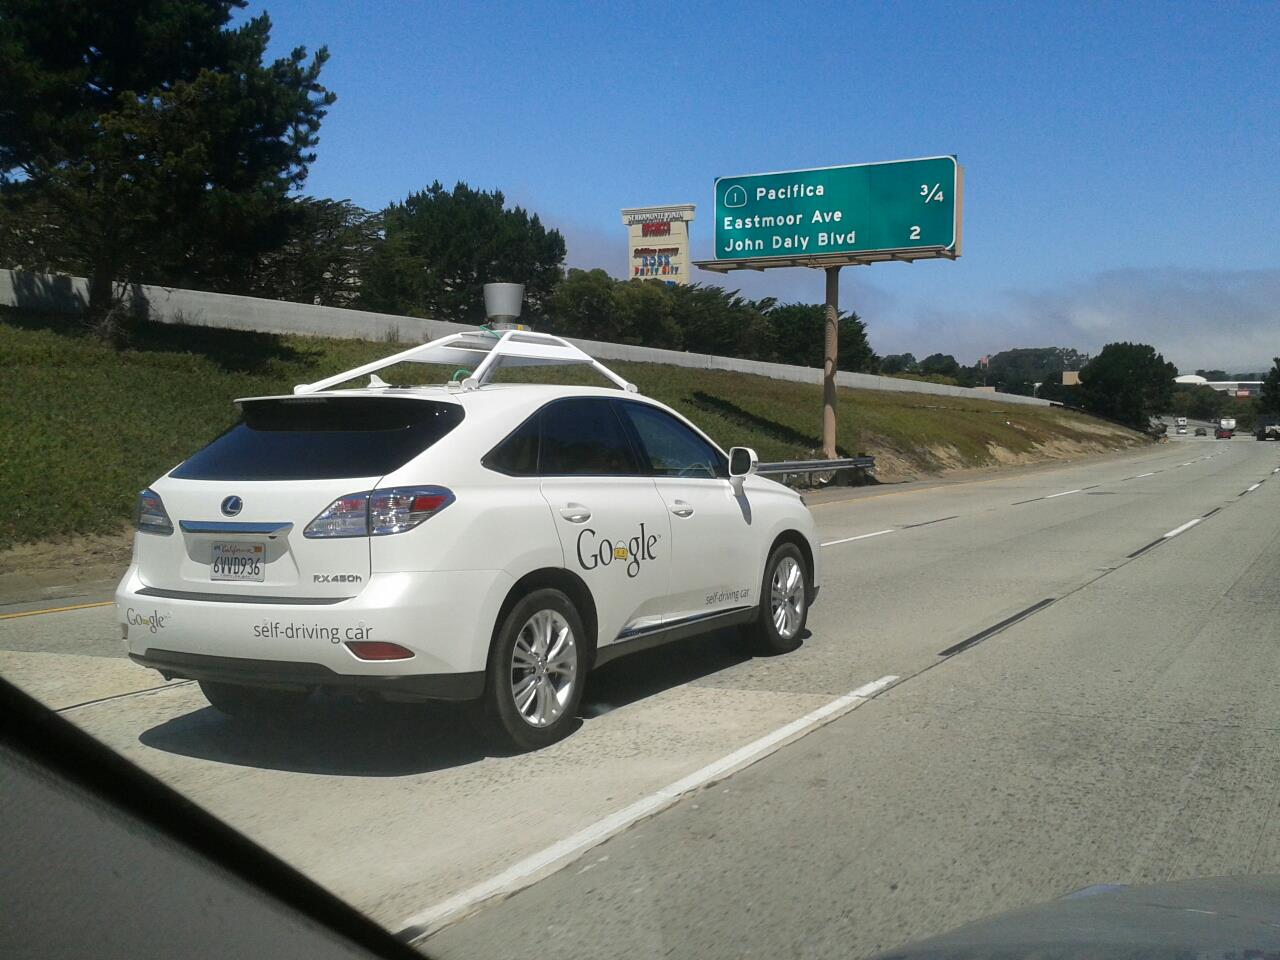
\includegraphics[height=2in]{google-self-driving-car.jpg}
        % Source: 
        %http://www.thetruthaboutcars.com/2013/01/self-driving-cars-the-legal-nitty-gritty/google-is-testing-out-their-self-driving-cars-imgur/
        %http://www.thetruthaboutcars.com/wp-content/uploads/2013/01/Google-is-testing-out-their-self-driving-cars-Imgur.jpg
        % License: ???
        % Date accessed: 1/11/2014        
        \caption*{Google self-driving car}
    \end{subfigure}
    \caption{Systems that are likely using Kalman filters or a variant thereof.}
\end{figure}


For vehicle guidance, navigation, and control, it is essential to know the state of the vehicle (location, orientation, velocity) of the vehicle at any given time. Usually, an array of sensors provides various kinds of information of varying quality (e.g., compass, accelerometers, gyroscope, GPS, vision, laser scanner), and this must be combined with knowledge of the vehicle's actions (e.g., wheels, propellors/turbines, rocket engines, ailerons), along with a physical model, in order to infer the state of the vehicle in real-time.  In 1960, Rudolf Kalman proposed a solution using a Bayesian time-series model which became known as the Kalman filter. The Kalman filter and its successors have been extraordinarily successful---it is difficult to overstate their importance in the guidance systems of aircraft, spacecraft, and robotics. 
% Also used in BCI for tracking desired hand position.

\subsection{Phylogenetics}

Understanding the evolutionary relationships among organisms---that is, the phylogenetic tree---is fundamental in nearly all biological research. Using genetic data from many organisms, along with models of how changes in the genome occur over time, researchers can infer the unknown evolutionary ``family tree''. Some of the dominant approaches use Bayesian inference (e.g., popular programs include MrBayes and BEAST) and these are widely used throughout biology. 

\begin{figure}
    \centering
        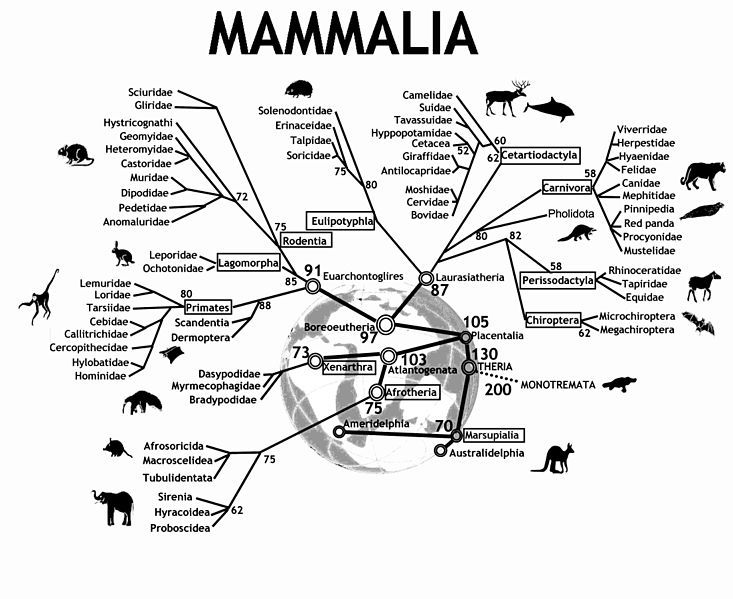
\includegraphics[trim=0 0 0 9,clip,width=0.9\textwidth]{An_evolutionary_tree_of_mammals.jpeg}
        % Source: http://commons.wikimedia.org/wiki/File:An_evolutionary_tree_of_mammals.jpeg
        %    Graphodatsky, Alexander S; Trifonov, Vladimir A; Stanyon, Roscoe (2011). "The genome diversity and karyotype evolution of mammals". Molecular Cytogenetics 4 (22).
        % License: This file is licensed under the Creative Commons Attribution 2.0 Generic license.
        % Date accessed: 1/11/2015
    \caption{Inferred phylogenetic tree of mammals. \scriptsize (Graphodatsky et al.\ 2011)}
\end{figure}



\subsection{Political science}

In 2008, Nate Silver correctly predicted the U.S. presidential election outcome in 49 out of 50 states, and in 2012, he got all 50 states right. Further, he predicted the U.S. Senate election outcome correctly in all 35 races in 2008, and in 31 of 33 races in 2012. Silver is an advocate of Bayesian statistics, and although the exact details are secret, it appears that he uses hierarchical Bayesian models to make his forecasts.\footnote{O'Hara, B. (2012). How did Nate Silver predict the US election? The Guardian. \url{http://www.theguardian.com/science/grrlscientist/2012/nov/08/nate-sliver-predict-us-election}}
Bayesian inference is also used extensively by other social science researchers in many other applications.

\begin{figure}
    \centering
        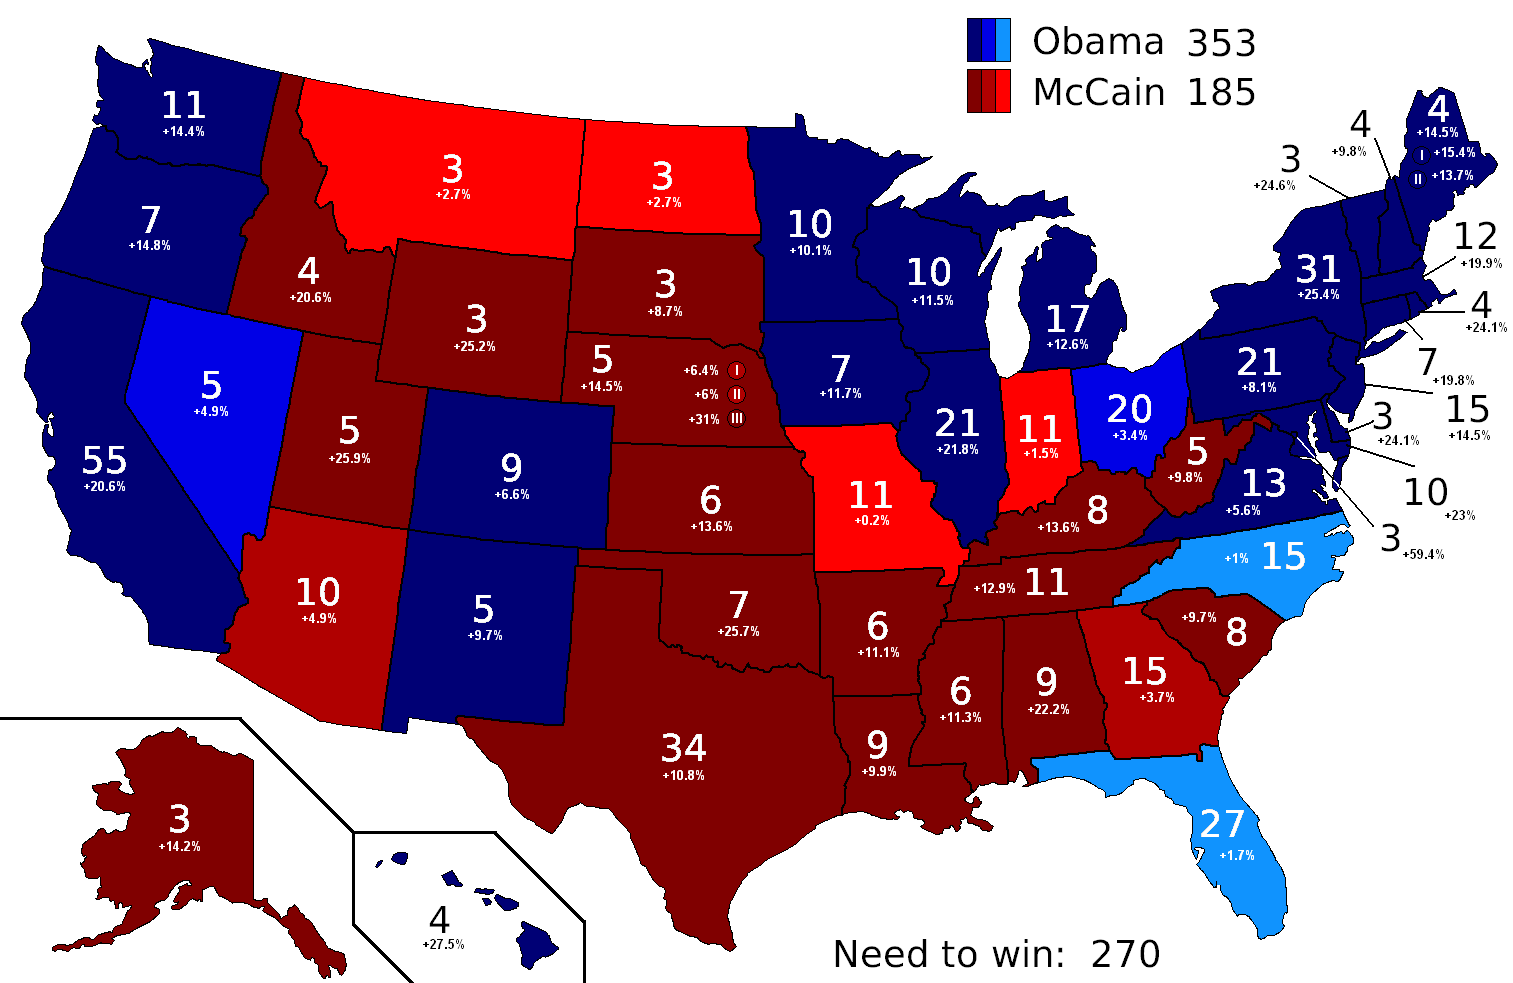
\includegraphics[width=0.8\textwidth]{fivethirtyeight.png}
        % Source: http://commons.wikimedia.org/wiki/File:Current_2008_US_Electoral_College_Polling_Map.PNG
        % License: Public domain
        % Date accessed: 1/11/2015
    \caption{Nate Silver's predictions for the 2008 presidential election.}
\end{figure}



\subsection{Computer science}

\begin{figure}
    \centering
        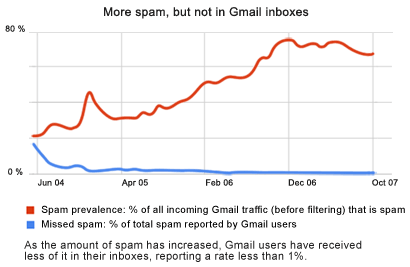
\includegraphics[width=0.65\textwidth]{spamchart.png}
        % Source: http://gmailblog.blogspot.com/2007/10/how-our-spam-filter-works.html
        % License: ???
        % Date accessed: 1/11/2015
    \caption{}
    \label{figure:spam}
\end{figure}

Spam accounts for the majority of email traffic---typically between 60 to 70\% of emails are spam.\footnote{Kaspersky Lab, Spam Statistics Reports: Figures, Sources, and Trending Data, 2013--2014. \url{http://usa.kaspersky.com/internet-security-center/threats/spam-statistics-reports-data}}
Yet, due to the sophisticated spam detection algorithms used by email service providers, very little spam gets through to your inbox---and only rarely is real mail classified as spam. For instance, in 2007, Gmail posted the chart in Figure \ref{figure:spam}, showing that the fraction of spam that gets through is very small indeed.\footnote{Jackson, T. (2007). How our spam filter works. \url{http://gmailblog.blogspot.com/2007/10/how-our-spam-filter-works.html}} Bayesian models are the most prominent methods for spam detection. A former Microsoft developer who moved to Google reportedly said, ``Google uses Bayesian filtering the way Microsoft uses the if statement.''\footnote{Joel on Software, Oct 17, 2005. \url{http://www.joelonsoftware.com/items/2005/10/17.html}}


\subsection{Search}

On June 1, 2009, Air France Flight 447 crashed into the Atlantic Ocean, killing all aboard. Despite three intensive searches, the underwater wreckage had still not been found a year later. French authorities were eventually able to recover the wreckage with the help of a Bayesian search analysis provided by the Metron company (Figure \ref{figure:AF447}). Bayesian search analysis involves formulating many hypothetical scenarios for what happened, constructing a probability distribution of the location under each scenario, and considering the posterior distribution on location given the searches conducted so far. It has also been used to find submarines and ships lost at sea.

\begin{figure}
    \centering
        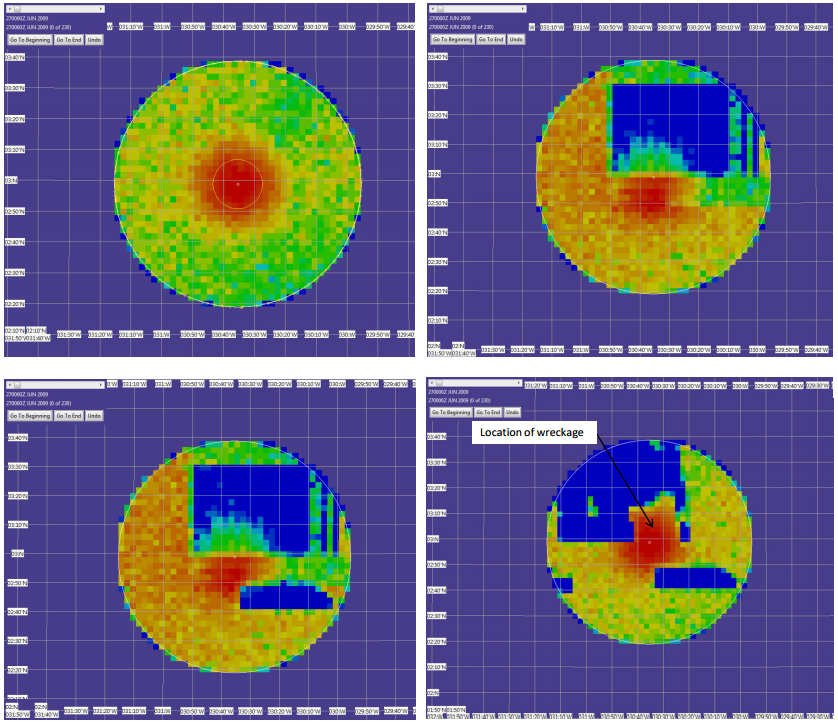
\includegraphics[width=0.7\textwidth]{AF447.png}     
        % Source: http://isif.org/fusion/proceedings/Fusion_2011/data/papers/140.pdf
        % Stone, L. D., Keller, C. M., Kratzke, T. M., & Strumpfer, J. P. (2011). Search analysis for the underwater wreckage of Air France Flight 447. In Information Fusion (FUSION), 2011 Proceedings of the 14th International Conference on (pp. 1-8). IEEE.
        % License: NEED TO ASK FOR PERMISSION TO PUBLISH. Fair use in lecture notes is OK.
        % Date accessed: 1/11/2015
        % Modifications: I trimmed some of the edges in order to make the sizes match, and combined the four figures.
    \caption{Prior and posteriors (after successive searches) for the location of the wreckage of Air France 447.  \scriptsize (Stone et al.\ 2011)}
    \label{figure:AF447}
\end{figure}


\subsection{Radiocarbon dating}

In archaeology, radiocarbon dating is often used to infer the age of an object. Many times, there is a significant amount of contextual knowledge that can also be brought to bear---for instance, other objects found nearby, where and how deep the object is found, constraints on the order of events, historical records, and other dating techniques. Bayesian methods are now being used to combine such different sources of information in order to improve the accuracy of radiocarbon dating.

\begin{figure}
    \centering
        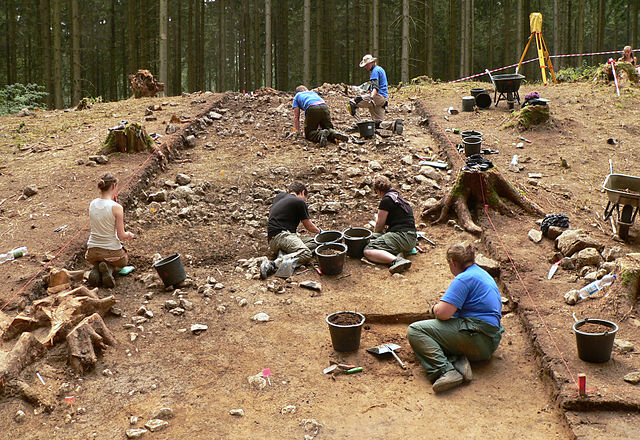
\includegraphics[width=0.7\textwidth]{archaeological-dig.jpg}     
        % Source: http://commons.wikimedia.org/wiki/File:Harzhorn_Grabungsschnitt_von_unten_1.jpg
        % License: This file is licensed under the Creative Commons Attribution 3.0 Unported license.
        % Date accessed: 1/12/2015
    \caption{An archaeological dig.  \scriptsize (Axel Hindemith)}
    \label{figure:archaeological-dig}
\end{figure}


% Gene expression --- empirical Bayes, Efron
% Econometrics
% Climate?
% Population structure (Pritchard) --- example: human populations study


\subsection{Many other applications as well}

This is just a small sampling of real-world applications in which Bayesian methods are actually used in practice. 




\section{What is Bayesian statistics?}

\subsubsection*{Bayes, in a nutshell}
The Bayesian approach can be summarized as follows:
\begin{quote}\small
Assume a probability distribution on any unknowns (this the prior), assume the distribution of the knowns given the unknowns (this is the generating distribution or likelihood), and then just follow the rules of probability to answer any questions of interest.
\end{quote}
An overarching theme of the Bayesian perspective is that uncertainty is quantified with probability distributions. Since essentially all statistical methods involve assuming the form of the generating distribution, it is the prior that distinguishes the Bayesian approach, and makes it possible to just follow the rules of probability.

\subsubsection*{Bayesian bubble of knowledge}
In essence, once distributions have been put on everything, a self-contained ``bubble of knowledge'' has been constructed in which the answer to any relevant question can---in principle---be answered in a probabilistic manner. The flipside, though, is that this bubble excludes many useful frequentist criteria for evaluating the performance of a procedure. It is important to evaluate Bayesian methods according to these other criteria as well.

\subsubsection*{What questions of interest often arise?}
Here are some recurring examples:
\begin{itemize}
\item estimate some unknown parameter or property,
\item infer hidden/latent variables or missing data,
\item predict future data,
\item test a hypothesis, or
\item choose among competing models.
\end{itemize}
In general, answering such questions can be viewed as a problem of choosing the optimal decision---and from our brief study of decision theory, we know that from the Bayesian perspective this consists of minimizing posterior expected loss.

%\subsection{The Big Picture}
\subsubsection*{How is this done? What methods are employed?}
In order to answer a question of interest, you usually have to get ahold of the posterior in one way or another, and compute one or more posterior expectations (integrals with respect to the posterior density). Three main categories of methods can be distinguished here: exact solution, deterministic approximation, and stochastic approximation.

\begin{enumerate}
\item \textbf{Exact solution}

In certain cases, it is computationally feasible to compute the posterior (and posterior expectations) exactly.
\begin{itemize}
\item Exponential families with conjugate priors often enable analytical solutions.
\item Gaussians, in particular, are highly conducive to analytical solutions.
\item For certain graphical models, dynamic programming can provide exact results.
\end{itemize}

\item \textbf{Deterministic approximation}

Methods include:
\begin{itemize}
\item numerical integration, a.k.a. quadrature/cubature
\item quasi-Monte Carlo (QMC), low discrepancy sequences
\item Laplace's method / Laplace approximation
\item expectation propagation (EP), variational Bayes (VB)
\end{itemize}
For low-dimensional integrals, numerical integration and QMC are superior to stochastic approximations. QMC can sometimes perform well in high-dimensional situations as well.

\item \textbf{Stochastic approximation}

For high-dimensional integrals, stochastic approximations are often the only option. The basic idea is that samples from the posterior can be used to approximate posterior expectations. Methods include:
\begin{itemize}
\item Monte Carlo approximation, importance sampling
\item Markov chain Monte Carlo (MCMC) --- Gibbs sampling, Metropolis algorithm, Metropolis--Hastings algorithm, slice sampling, Hamiltonian MCMC
\item sequential importance sampling, sequential Monte Carlo, population Monte Carlo
\item approximate Bayesian computation (ABC)
\end{itemize}
\end{enumerate}


\vspace{2em}

\section{What is the difference between the Bayesian and frequentist perspectives?}
%\subsection{Contrast with the frequentist perspective}

Once you understand it, the Bayesian approach seems so natural that it is hard to imagine any alternative. In fact, there was no satisfying alternative until the early 1900's, when Karl Pearson, Jerzy Neyman, Egon Pearson, and Ronald Fisher initiated what is now called frequentist statistics. %(See Section \ref{section:history} for more on the history.)

Roughly, the essential difference between the Bayesian and frequentist perspectives can be described as follows, letting $x$ denote the observed data, and $\theta$ denote the unknowns:
\begin{itemize}
\item the Bayesian considers only the observed value of $x$, and treats $\theta$ as random,
\item the frequentist considers all possible values of $x$, and treats $\theta$ as fixed.
\end{itemize}
The Bayesian approach is to make the best possible decision given observations $x$, allowing for uncertainty in $\theta$. The frequentist approach is to use a decision procedure that will have guaranteed performance when used repeatedly, no matter what $\theta$ turns out to be.


\subsection{Example: Diagnosing celiac disease}
\label{section:celiac}
Approximately 1 in 100 people is affected by celiac disease, an autoimmune disorder resulting in sensitivity to gluten. Initial diagnosis of the disease is often made using a blood test that measures the level $x$ of a certain antibody. If $x$ is above a certain cutoff point, then a positive diagnosis is made (i.e., disease is present), otherwise, a negative diagnosis is made (i.e., disease not present).\footnote{This description is slightly simplified, for illustration purposes.}
%(immunoglobulin A anti-tissue transglutaminase)

How should this cutoff point be chosen? If the cutoff is too low, there will be too many false positives (incorrectly diagnosing a person as diseased), while if it is too high, there will be too many false negatives (incorrectly diagnosing as undiseased).
% unnecessary resulting in further testing which is physically uncomfortable, mental distress, and financial expense. 
Given $x$, we are faced with the following hypothesis testing problem.
\begin{quote}
Hypothesis 0 ($\theta_0$): Undiseased. \\
Hypothesis 1 ($\theta_1$): Diseased.
\end{quote}
% In a situation like this where there are two competing hypotheses, one of which is the ``default'' ($\theta_0$), and one of which is the ``challenger'' ($\theta_1$), it is customary to refer to $\theta_0$ as the \term{null hypothesis} and $\theta_1$ as the \term{alternative hypothesis}.
% There are two types of errors we can make:
% \begin{enumerate}
% \item \term{Type I errors} / \term{false positives}, in which we choose $\theta_1$ when $\theta_0$ is true, or
% \item \term{Type II errors} / \term{false negatives}, in which we choose $\theta_0$ when $\theta_1$ is true.
% \end{enumerate}
% Depending on the situation, the loss function may penalize each type of error differently.
Suppose that from many previous cases, we know the distributions $p(x|\theta_0)$ and $p(x|\theta_1)$ of the antibody level $x$ for undiseased and diseased individuals, respectively. 

\subsubsection*{Bayesian approach}

The Bayesian approach is as follows. Since 1 in 100 people is affected, we have $p(\theta_1) = 1/100$ (and thus $p(\theta_0) = 99/100$); this is the prior. Using Bayes' theorem, we can compute the posterior probability of disease for a given individual,
$$ p(\theta_1|x) =\frac{p(x|\theta_1) p(\theta_1)}{p(x|\theta_0) p(\theta_0) + p(x|\theta_1) p(\theta_1)}. $$
Quantifying each possible outcome in terms of a loss function $\ell$, a diagnosis ($a=\theta_0$ or $a=\theta_1$) is made to minimize the posterior expected loss,
$$ \rho(a,x) = \ell(\theta_0,a) p(\theta_0|x) + \ell(\theta_1,a) p(\theta_1|x). $$

\subsubsection*{Frequentist approach}

The usual frequentist approach, on the other hand, is to use a decision procedure that minimizes false negatives, subject to an upper bound on false positives, say, $\alpha = 0.05$. 
Due to a result called the Neyman--Pearson lemma, this is achieved by choosing $a=\theta_1$ when
$$\frac{p(x|\theta_1)}{p(x|\theta_0)}>c $$
and $a =\theta_0$ otherwise, where $c\geq 0$ is chosen so that the probability of a false positive equals $\alpha$, i.e.,
% $$\Pr\left(\frac{p(X|\theta_1)}{p(X|\theta_0)}>c \,\,\middle| \,\, \theta_0\right) = \alpha.$$
$$\Pr(X\in R_c\mid\theta_0) = \int_{R_c} p(x|\theta_0) d x  = \alpha$$
where $R_c = \big\{x: p(x|\theta_1)/p(x|\theta_0)>c\big\}$.

\subsubsection*{Comparing the two approaches}

So, in the Bayesian approach, the unknown state (diseased or undiseased) is treated as a random variable (since we put a prior on it), and we only consider the observed value of $x$ throughout the analysis. Meanwhile, in the frequentist approach, no prior is used, and the decision procedure (specifically, the choice of $c$) depends on considering all possible values of the observation $x$.

The Bayesian approach is optimal under the assumed prior and loss, while the frequentist approach is optimal subject to the chosen bound on false positives.

In a binary decision such as this, it turns out that the two approaches are equivalent, in the sense that for any prior and loss, there is a choice of $c$ for which the Neyman--Pearson procedure coincides with the Bayes procedure---and vice versa, for any $c$ there is a prior and loss for which they coincide.

%\textbf{Estimation: What is the antibody level?}



\subsection{Further contrasts between Bayesian and frequentist}

\subsubsection*{Interpretation of probability}
From the frequentist perspective, the true value of $\theta$ is some unknown but fixed quantity, and it doesn't make sense to speak of $\theta$ having a probability distribution---for instance, in the disease diagnosis example of Section \ref{section:celiac}, the patient either has the disease or doesn't, so the probability that the patient has the disease is either 1 or 0.  

In order for the Bayesian perspective to make sense, a probability must be interpreted as a subjective level of belief in the truth of a proposition. 
In contrast, the frequentist interpretation of probability is empirical: the probability of an outcome is the fraction of times it would occur in a sequence of infinitely many trials. (Note: A common misconception is that the frequentist definition only makes sense for trials that have actually occurred many times in the real world, but this is wrong---the trials can be hypothetical.)

\subsubsection*{Coherence versus calibration}
An appealing aspect of the Bayesian approach is its coherence---that is, once the prior has been assumed, no contradictions will arise in the course of doing inference. However, if the prior or likelihood is chosen poorly, this simply means the inferences will be consistently wrong.

Meanwhile, an attractive feature of the frequentist approach is calibration guarantees---that is, we can specify certain performance characteristics, and be guaranteed that they will be met if the procedure is used many times. For instance, in the disease diagnosis example, we specify the fraction of false positives $\alpha=0.05$, and it is guaranteed that this will be the fraction of false positives occurring in practice (assuming the model is correct).

% One of the most common frequentist criticisms of the Bayesian approach is that correct calibration is not guaranteed. However, it should be noted that many frequentist methods use approximations for which calibration is only guaranteed asymptotically.

\subsubsection*{Frequentist evaluations}
From the purely Bayesian perspective, if the prior and likelihood are chosen properly, then the resulting inferences are correct and optimal, and there is nothing more to be said. However, in practice this is not very satisfying, since we often:
\begin{itemize}
\item are uncertain about the choice of prior or likelihood,
\item employ approximations, and
\item want methods which perform well in a wide variety of circumstances.
\end{itemize}
The frequentist perspective provides empirical and theoretical tools to deal with these issues. Empirically, one can assess performance using cross-validation, test sets, bootstrap, goodness-of-fit tests, and posterior predictive checks. Theoretically, one can provide guarantees of consistency (i.e., convergence to the true value), rates of convergence, and calibration/coverage.

It is a common misconception that the Bayesian and frequentist approaches are mutually exclusive, but this is  incorrect. From the frequentist perspective, any procedure can be used---including a Bayesian one---if you can prove that it does what you want.


\subsection{Overall recommendation: be pragmatic, not dogmatic}

Overall, be pragmatic---that is, use what has been shown to work.
As a default approach, the following will serve you well:
\begin{quote}
\textit{Design as a Bayesian, and evaluate as a frequentist.}
\end{quote}
In other words, construct models and procedures from a Bayesian perspective, and use frequentist tools to evaluate their empirical and theoretical performance. In the spirit of being pragmatic, it might seem unnecessarily restrictive to limit oneself to Bayesian procedures, and indeed, there are times when a non-Bayesian procedure may be preferable to a Bayesian one. However, typically, it turns out that there is no disadvantage in considering only Bayesian procedures---this has been shown formally via the ``complete class theorems''.

%, as we will discuss in Section \ref{section:why}.


% In non-trivial problems, it is a bit odd to accept the generating distribution without question, and balk at the subjectivity of the prior. The choice of generating distribution has a much stronger influence on the outcome than does the prior.

% Default recommendation (inherited from Matt Harrison):
% As a default approach, this will serve you well: "Bayesian design, frequentist assessment."
% - Use Bayes for design/implementation
    % - model building, inference, decision-making
% - Use Frequentist for evaluation/assessment
    % - Theoretical
        % - consistency, rates of convergence, asymptotic distribution
    % - Empirical
        % - cross-validation, held-out tests sets, etc. (other examples?)
        % - model checking

% However, there are times when a frequentist proc. may be preferable to a Bayesian one.

% My overall take: "Be pragmatic, not dogmatic." (Use what has been shown to work.)





%\section{Why use Bayesian methods? Advantages and disadvantages.}
%\label{section:why}


% It should also be noted that there are also times when using a Bayesian procedure is not worth the trouble, since a simple non-Bayesian procedure is easy to use and gives sufficiently good performance.

%\section{A brief history of statistics}
%\label{section:history}




%\section*{Exercises}

% \item Show that in the example of Section \ref{section:celiac}, for any prior and loss, there is a choice of $c$ for which the Bayes procedure coincides with the Neyman--Pearson procedure.






\section*{References and supplements}

\subsubsection*{Applications}
\begin{itemize}
\item Kalman, R. E. (1960). A new approach to linear filtering and prediction problems. Journal of Basic Engineering, 82(1), 35-45.
\item O'Leary, M. A., et al.\ (2013). The placental mammal ancestor and the post�K-Pg radiation of placentals. Science, 339(6120), 662-667.
\item Graphodatsky, A. S., Trifonov, V. A., \& Stanyon, R. (2011). The genome diversity and karyotype evolution of mammals. Mol Cytogenet, 4(1), 22.
\item Stone, L. D., Keller, C. M., Kratzke, T. M., \& Strumpfer, J. P. (2011). Search analysis for the underwater wreckage of Air France Flight 447. In Information Fusion (FUSION), 2011 Proceedings of the 14th International Conference on (pp. 1-8). IEEE.
\item Ramsey, C. B. (2009). Bayesian analysis of radiocarbon dates. Radiocarbon, 51(1), 337-360.
\end{itemize}

\subsubsection*{Frequentist and Bayesian}
\begin{itemize}
\item Kass, R. E. (2011). Statistical inference: The big picture. Statistical Science, 26(1), 1. \url{http://projecteuclid.org/euclid.ss/1307626554}
\item Jordan, M. I.  Are You a Bayesian or a Frequentist? (2009) \url{http://videolectures.net/mlss09uk_jordan_bfway/}
\end{itemize}


\end{document}






